\documentclass[12pt]{article}
\usepackage{graphicx}

%opening
\title{A Step by Step Backpropagation Example}
\author{Luigi Russo}

\begin{document}

\maketitle

\section{Overview}
This is a very simple example, strongly inspired by M. Mazur's article \cite{articolo}, that attempts to explain how backpropagation works. I tried to make it as concrete as possible, going through all phases of the algorithm.
I am going to use a neural network with three inputs, three hidden neurons, three output neurons; additionally, the hidden and output neurons will include a bias.
In order to make this example handier, I am going to assign numerical values (precision
\begin{math}
10^{-5}
\end{math}) to the initial weights, the biases, and training inputs/outputs.
\begin{center}
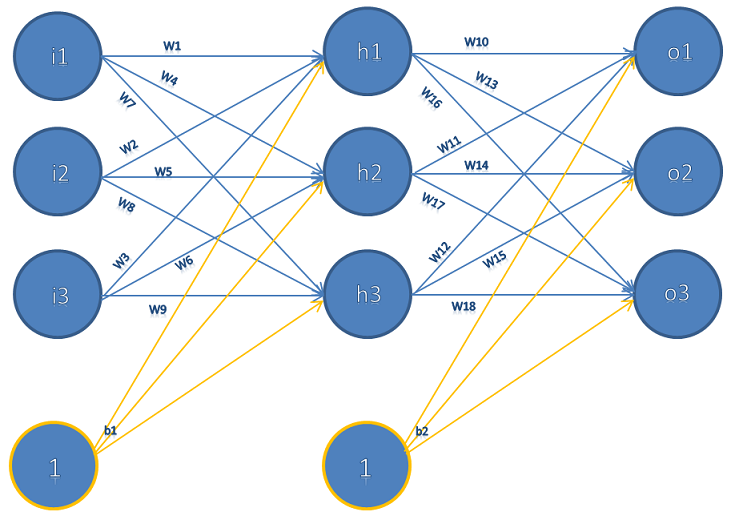
\includegraphics[width=350pt, keepaspectratio]{image.png}
\end{center}

\section{The Forward Pass}
To begin, we want to see what the neural network currently predicts given some weights, bias and inputs values. First of all, we need to set these values and we can later feed inputs forward though the network.\\
For all this \textit{excercise} I am going to work with a single training set: given inputs i1, i2, 13 I want the neural network to output some \textbf{fixed} o1, o2, o3.
\subsection{Initial settings}
Let's set values!\\
For inputs:\\
i1 = 0.05, i2 = 0.1, i3 = 0.15\\
For weights:\\
w1 = 0.2, w2 = 0.25, w3 = 0.3\\
w4 = 0.35, w5 = 0.4, w6 = 0.45\\
w7 = 0.5, w8 = 0.55, w9 = 0.6\\
w10 = 0.65, w11 = 0.7, w12 = 0.75\\
w13 = 0.8, w14 = 0.85, w15 = 0.9\\
w16 = 0.1, w17 = 0.2, w18 = 0.3\\
For bias:\\
b1 = 0.3, b2 = 0.6\\
For outputs:\\
o1 = 0.1, o2 = 0.5, 03 = 0.9
\subsection{First feed}
Here is how we calculate the total net input for 
\begin{math}
h_1:\newline\newline
net_{h1} = w_1 * i_1 + w_2 * i_2 + w_3 * i_3 + b_1 * 1 = 0.38\newline\newline
out_{h1} = \frac{1}{1 + e^{- net_{h1}}} = 0.59387\newline\newline
\end{math}
This way we also get 
\begin{math}out_{h2} = 0.60468 \end{math} 
and 
\begin{math}out_{h3} = 0.61538\end{math}.
Repeating this process for the output layer neurons and using the output from the hidden layer neurons as inputs we have for
\begin{math}
o_{1}:\newline\newline
net_{o1} = w_{10} * out_{h1} + w_{11} * out_{h2} + w_{12} * out_{h3} + b_2 * 1 = 1.87083 \newline\newline
out_{o1} = \frac{1}{1 + e^{- net_{o1}}} = 0.86655\newline\newline
\end{math}
This way we also get 
\begin{math}out_{o2} = 0.895\end{math} 
and 
\begin{math}out_{o3} = 0.72411\end{math} 
\subsection{Calculating the error}
We can now calculate the total error:
\begin{math}
\newline\newline
E_{total} = \frac{1}{2} [target - output]^{T}[target - output] = 0.38728\newline\newline
\end{math}
It can be also seen as sum of three components: 
\begin{math}
E_{total} = E_{o1} + E_{o2} + E_{o3}
\end{math}
where
\begin{math}
E_{oi} = \frac{1}{2} (target_{oi} - output_{oi})^{2}, i \in (1,2,3)\newline
\end{math}
In particular:
\begin{math}
\newline\newline
E_{o1} = 0.2938, E_{o2} = 0.07801, E_{o3} = 0.01547
\end{math}
\section{The Backward Pass}
The goal with backpropagation is to update each of the weights in the network so that they cause the actual output to be closer the target output, thereby minimizing the total error.
\subsection{The output layer}
Consider 
\begin{math}w_{10}\end{math}.
We want to know how much a change in 
\begin{math}w_{10}\end{math} 
affects the total error, i.e.  
\begin{math}
\frac{\partial E_{total}}{\partial w_{10}}
\end{math}
By applying the chain rule we know that:
\begin{math}
\newline\newline
\frac{\partial E_{total}}{\partial w_{10}} = \frac{\partial E_{total}}{\partial out_{o1}} * \frac{\partial out_{o1}}{\partial net_{o1}} * \frac{\partial net_{o1}}{\partial w_{10}}
\newline\newline
\end{math}
First, this is how much the total error changes with respect to the output
\begin{math}
\newline\newline
\frac{\partial E_{total}}{\partial out_{o1}} = out_{o1} - target_{o1} = 0.76655
\newline\newline
\end{math}
Second, this is how much the output of
\begin{math}o_1\end{math}
changes with respect to its total net input?
\begin{math}
\newline\newline
\frac{\partial out_{o1}}{\partial net_{o1}} = out_{o1}(1 - out_{o1}) = 0.11564
\newline\newline
\end{math}
Thirs, this is how much the total net input of o1 changes with respect to 
\begin{math}w_{10}?
\newline\newline
\frac{\partial net_{o1}}{\partial w_{10}} = out_{h1} = 0.59387
\newline\newline
\end{math}
Putting it all together:
\begin{math}
\newline\newline
\frac{\partial E_{total}}{\partial w_{10}} = \frac{\partial E_{total}}{\partial out_{o1}} * \frac{\partial out_{o1}}{\partial net_{o1}} * \frac{\partial net_{o1}}{\partial w_{10}} = 0.05304
\newline\newline
\end{math}
To decrease the error, we then subtract this value from the current weight (optionally multiplied by some learning rate
\begin{math}\eta\end{math}, which we set to 0.5):
\begin{math}
\newline\newline
w_{10}^{n} = w_{10} - \eta * \frac{\partial E_{total}}{\partial w_{10}} = 0.65 - 0.5 * 0.05304 = 0.62348
\newline\newline
\end{math}
Repeating this process we get the new weights:
\begin{math}
\newline
w_{11}^{n} = 0.6732, w_{12}^{n} = 0.72272, w_{13}^{n} = 0.78897, w_{14}^{n} = 0.83877, w_{15}^{n} = 0.88858,
\newline
w_{16}^{n} = 0.11043, w_{17}^{n} = 0.21062, w_{18}^{n} = 0.31081
\newline\newline
\end{math}
\textbf{Note:} It is important to use the original weights, not the updated weights, when we continue the backpropagation algorithm below.

\subsection{The hidden layer}
The goal of this subsection is to update the weights that are between inputs and hidden neurons. Let us consider
\begin{math}w_1.
\newline\newline
\frac{\partial E_{total}}{\partial w_{1}} = \frac{\partial E_{total}}{\partial out_{h1}} * \frac{\partial out_{h1}}{\partial net_{h1}} * \frac{\partial net_{h1}}{\partial w_{1}}
\newline\newline
\end{math}
where
\begin{math}
\frac{\partial E_{total}}{\partial out_{h1}} = \frac{\partial E_{o1}}{\partial out_{h1}} + \frac{\partial E_{o2}}{\partial out_{h1}} + \frac{\partial E_{o3}}{\partial out_{h1}}
\newline\newline
\end{math}
Starting with
\begin{math}
\frac{\partial E_{o1}}{\partial out_{h1}}:
\newline\newline
\frac{\partial E_{o1}}{\partial out_{h1}} = \frac{\partial E_{o1}}{\partial net_{o1}} * \frac{\partial net_{o1}}{\partial out_{h1}} = \frac{\partial E_{o1}}{\partial out_{o1}} * \frac{\partial out_{o1}}{\partial net_{o1}} * w_{10} = 0.057618
\newline\newline
\end{math}
In a similar way we get
\begin{math}
\frac{\partial E_{o2}}{\partial out_{h1}} = 0.0297, \frac{\partial E_{o3}}{\partial out_{h1}} = -0.00351
\newline\newline
\end{math}
Therefore:
\begin{math}
\newline\newline
\frac{\partial E_{total}}{\partial out_{h1}} = \frac{\partial E_{o1}}{\partial out_{h1}} + \frac{\partial E_{o2}}{\partial out_{h1}} + \frac{\partial E_{o3}}{\partial out_{h1}} = 0.08381
\newline\newline
\end{math}
Considering that
\begin{math}
\newline\newline
(i)\;\; \frac{\partial out_{h1}}{\partial net_{h1}} = out_{h1}(1 - out_{h1}) = 0.24119
\newline\newline
(ii)\; \frac{\partial net_{h1}}{\partial w_1} = i_1 = 0.05
\newline\newline
\end{math}
we can finally get:
\begin{math}
\newline\newline
\frac{\partial E_{total}}{\partial w_{1}} = \frac{\partial E_{total}}{\partial out_{h1}} * \frac{\partial out_{h1}}{\partial net_{h1}} * \frac{\partial net_{h1}}{\partial w_{1}} = 0.00101
\newline\newline
\end{math}
We can now update the weights:
\begin{math}
\newline\newline
w_1^{n} = w_1 - \eta * \frac{\partial E_{total}}{\partial w_{1}} = 0.19949
\newline\newline
\end{math}
Repeating this process we get the new weights:
\begin{math}
\newline
w_{2}^{n} = 0.24899, w_{3}^{n} = 0.29848, w_{4}^{n} = 0.34948, w_{5}^{n} = 0.39845, w_{6}^{n} = 0.44845,\newline
w_{7}^{n} = 0.49947, w_{8}^{n} = 0.54894, w_{9}^{n} = 0.59841
\end{math}
\section{The forward pass. Again}
Finally, all weights have been updated.
Feeding forward the inputs in the updated network we get:
\begin{math}
\newline\newline
out_{h1} = 0.59379, out_{h2} = 0.60458, out_{h3} = 0.62237\newline
out_{o1} = 0.86141, out_{o2} = 0.89365, out_{o3} = 0.72837
\newline\newline
\end{math}
When we fed forward the inputs originally, the error on the network was 0.38728. After this first round of backpropagation, the total error is now down to 0.38208, i.e error was reduced by \textbf{0,0052}
\section{Conclusions}
It might not seem like much, but the process described above must be iterated several times to get total error quite close to 0. I strongly suggest to use a script \cite{repo-git} to do that.
\begin{thebibliography}{2}
\bibitem{articolo}
M. Mazur.
\textit{A Step by Step Backpropagation Example. \\\texttt{https://www.mattmazur.com} , March 17, 2015}

\bibitem{repo-git}
M. Mazur.
\textit{Backpropagation Algorithm in Python. \\\texttt{https://github.com/mattm/simple-neural-network}}
\end{thebibliography}

\end{document}
